\subsubsection{Software del servidor}
Para la visualización y representación de los distintos valores de tensión y corriente medidos por los diferentes sensores, se ha optado por utilizar ThingsBoard, una plataforma IoT de código abierto para la recopilación, el procesamiento, la visualización y la gestión de dispositivos de datos.

\begin{figure}[H]
    \centering
    
\includegraphics[width=0.3\textwidth]{images/3-software/3-2-2-thingsboard/LogoThingsboard.png}
    \caption{Plataforma ThingsBoard}
    \label{fig:3-2-2-ThingsBoard}
\end{figure}

Para su instalación en el ordenador, se ha optado utilizar una máquina virtual en VirtualBox mediante la imagen de un servidor Linux con distribución Ubuntu.
Debido al uso de dicha maquina virtual, se ha tenido que realizar una redirección de los puertos mediante la interfaz de red de la propia máquina, obteniendo la siguiente configuración:

\begin{figure}[H]
    \centering
    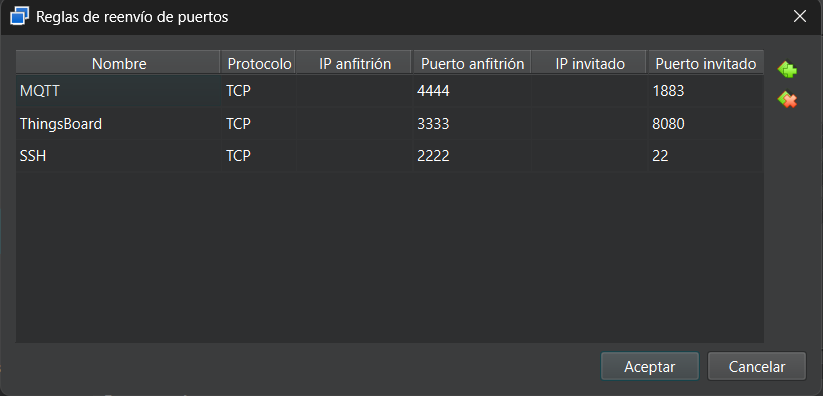
\includegraphics[width=0.3\textwidth]{images/3-software/3-2-2-thingsboard/PuertosMV.png}
    \caption{Redirección de puertos MV}
    \label{fig:3-2-2-PuertosMV}
\end{figure}

Para la visualización de los datos recibido, se ha optado por diseñar dos paneles o \textit{Dashboards}, uno en representación en forma de tablas y otro en forma de gráficas. Ambos paneles se actualizan en tiempo real y cuentan con una tabla o gráfica para cada dispositivo, obtenido un total de 4 tablas y 4 gráficas. Además, en las gráficas se puede visualizar también la media de los últimos datos medidos.

\begin{figure}[H]
    \centering
    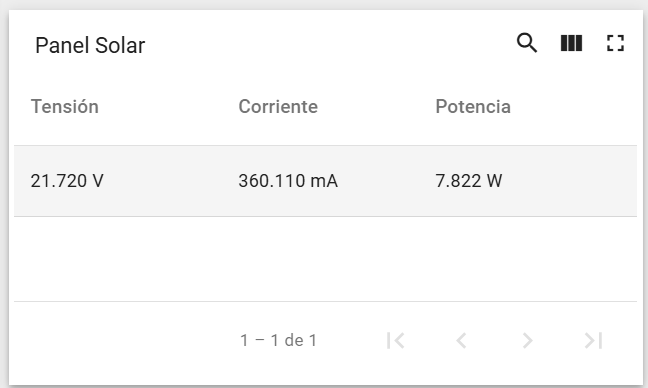
\includegraphics[width=0.3\textwidth]{images/3-software/3-2-2-thingsboard/TablaThingsBoard.png}
    \caption{Tabla de medidas}
    \label{fig:3-2-2-TablaThingsBoard}
\end{figure}

\begin{figure}[H]
    \centering
    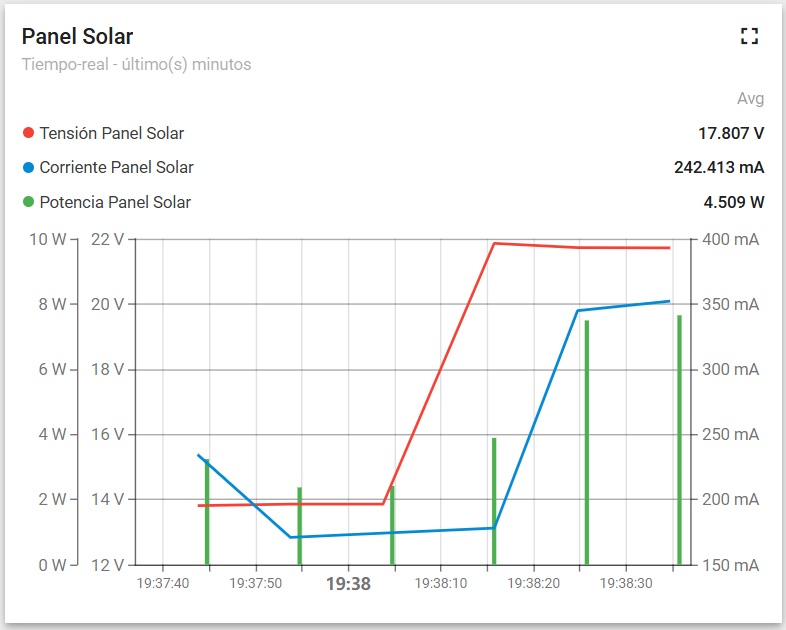
\includegraphics[width=0.3\textwidth]{images/3-software/3-2-2-thingsboard/GraficaThingsBoard.png}
    \caption{Gráfica de medidas}
    \label{fig:3-2-2-GraficaThingsBoard}
\end{figure}

Debido a que mediante los sensores solo se obtienen valores de tensión y de corriente, se ha implementado un algoritmo mediante las cadenas de reglas de Thingsboard. Se ha necesitado crear una cadena de reglas para cada potencia calculada, obteniendo 4 cadena de reglas como la siguiente:

\begin{figure}[H]
    \centering
    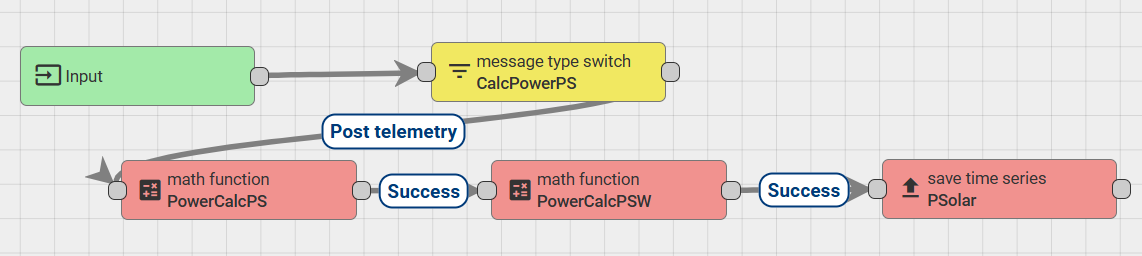
\includegraphics[width=0.3\textwidth]{images/3-software/3-2-2-thingsboard/CadenaPotencia.png}
    \caption{Cadena de reglas para cálculo de potencias}
    \label{fig:3-2-2-CadenaPotenciaThingsBoard}
\end{figure}

Dichas cadenas de reglas se dividen en los siguientes pasos:

\begin{enumerate}
    \item Filtrar y transformar la telemetría entrante
    \item Realizar el cálculo de la potencia correspondiente
    \item Pasar dicha potencia a Vatios
    \item Guardas los valores para su reprentación
\end{enumerate}

Por último, se ha añadido dichas cadenas de reglas de potencia a la cadena de regla principal, la cual gestiona el funcionamiento completo de Thingsboard y permite visualizar el dato obtenido de su respectiva cadena de regla.

\begin{figure}[H]
    \centering
    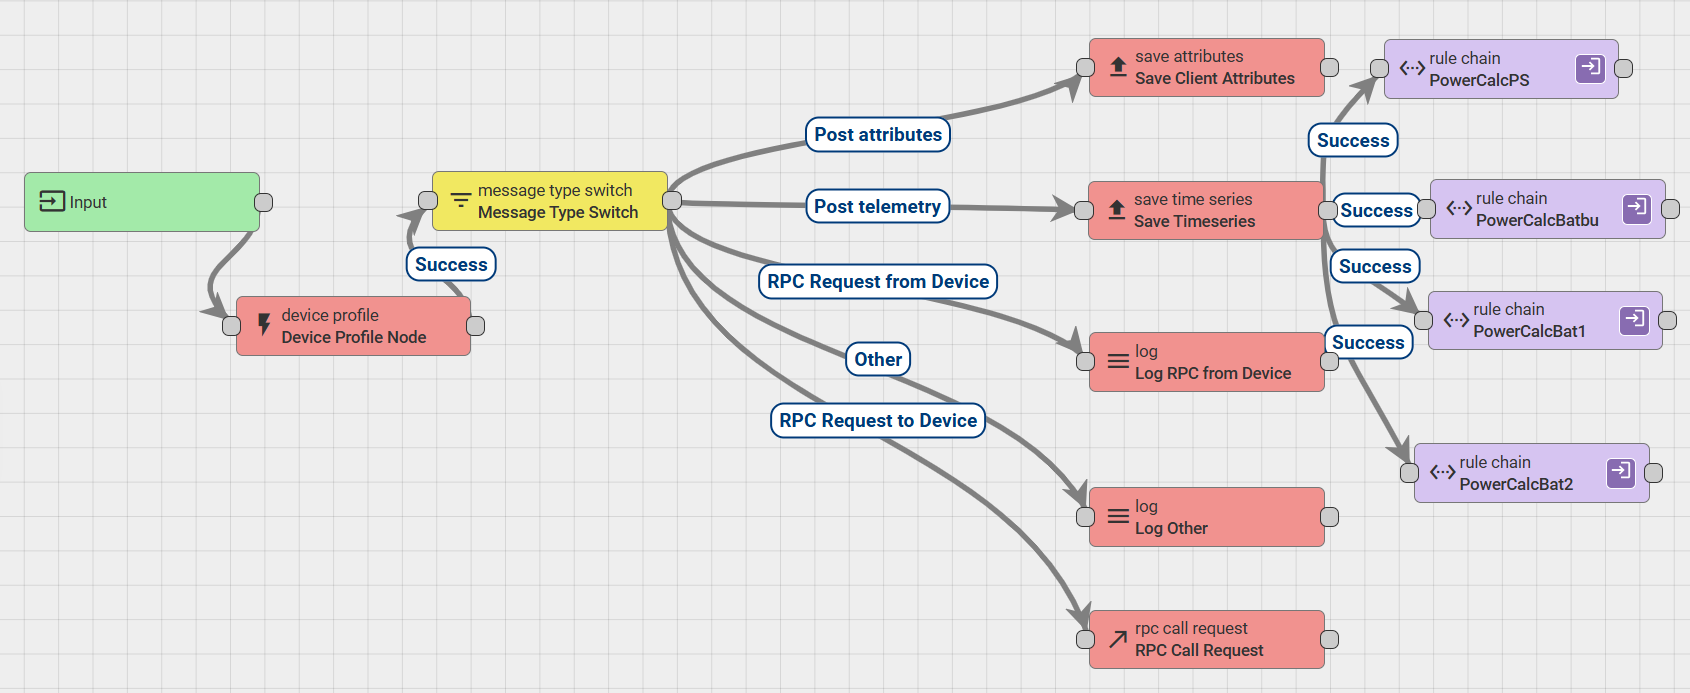
\includegraphics[width=0.3\textwidth]{images/3-software/3-2-2-thingsboard/CadenaPrincipal.png}
    \caption{Cadena de reglas principal}
    \label{fig:3-2-2-CadenaPrincipalThingsBoard}
\end{figure}